\section{Verteilte Publish/Subscribe-Systeme}
\label{chap:grundlagen:pubsub}
Diese Arbeit beschäftigt sich ausschließlich mit dezentralen Publish/Subscribe-Sys\-temen, denn \ac{m2etis} zielt darauf ab, die Rechner der Nutzer in einem p2p-Netzwerk zu verbinden und darauf aufbauend die Events in einem Publish/Subscribe-System zu verteilen. Viele der Grundlagen in diesem Kapitel gelten sowohl für klassische zentrale wie auch dezentrale Publish/Subscribe-Systeme, allerdings müssen im verteilten Fall die Verwaltungsinformationen dezentral auf allen Knoten gespeichert werden, beziehungsweise geeignete Verteilunsalgorithmen gefunden werden. Ausgefallene Knoten können aktiv anhand von periodischen \enquote{heartbeat}-Nachrichten erkannt werden. Allerdings ist eine periodische Neuanmeldung der Subscriber von Vorteil, da hier die Subscribe-Nachrichten vom Netzwerk automatisch über andere Knoten geleitet werden und sich so der logische Verteilungsbaum wieder aufbauen kann. Die meisten verteilten Publish/Subscribe-Systemem fordern daher eine periodische Auffrischung der Anmeldungen eines Knotens.\\
Liu gibt einen Überblick über diese Systeme \cite{Liu2003Survey} während Banerjee verschiedene Protokolle in Multicast-Systemen vergleicht und den \enquote{Multicast-Tree'' als Verteilungssystem vorstellt \cite{Banerjee2001Comparative}. Sicherheit \cite{FiegeSecurity}, ``Quality of Service} \cite{BeFiMu2006PubSubQoS} oder Verteilungsoptimierung \cite{Muhl2002LargeScale} sind ebenfalls Forschungsthemen und ausführlich bearbeitet.

Konzeptionell lassen sich Publish/Subscribe-Systeme als eventbasierte Systeme betrachten. Auf Grund ihres Aufbaus und der Skalierung  in orthogonalen Dimensionen\index{Publish/Subscribe!orthogonale Dimensionen} \enquote{Raum'', ``Zeit'' sowie ``Verarbeitungsmodell} eignen sich diese gut zur Verteilung von Events in dezentralen Umgebungen \cite{PatrickTh2003Many, Cugola2002Using}.

\begin{figure}[htbp]
\centering
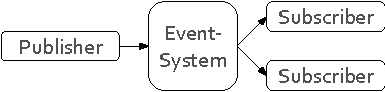
\includegraphics{grafics/pubsub_black_box.pdf}
\caption{Schema eines Publish/Subscribe-Systemes.}
\label{fig:pubsub_black_box}
\end{figure}

Publisher und Subscriber werden durch das Event-System voneinander getrennt, wie es in \Fref{fig:pubsub_black_box} dargestellt ist. Diese Trennung bezieht sich nicht nur auf verschiedene Komponenten einer Applikation, sondern kann auch über Applikations- oder gar Rechnergrenzen gehen. Publisher und Subscriber sind in ihren Aktionen mit dem Event-System zeitlich getrennt und sie müssen kein Wissen voneinander haben. Dies bedeutet dass sich ein Subscriber am System anmelden kann obwohl kein Publisher vorhanden ist, analog können Nachrichten publiziert werden ohne dass Empfänger eingeschrieben sind. Bei einem Fernaufrufsystem wie \emph{remote proceduce call (RPC)} \cite{Birrell1984Implementing} ist dies nicht möglich, da die Gegenseite bekannt sein muss. Das Senden einer Nachricht ist für den Publisher nicht blockierend und entspricht dem Kommunikationsparadigma \enquote{send and forget}. Subscriber warten zudem nicht aktiv auf neue Nachrichten, sondern werden meist per Callback über neue Nachrichten informiert. Damit wird die Verarbeitung vom Event-System aus getriggert.

Publish/Subscribe-Systeme lassen sich grundsätzlich in zwei Varianten einteilen: \emph{kanalbasiert}\index{Publish/Subscribe!kanalbasiert} und \emph{filterbasiert}\index{Publish/Subscribe!filterbasiert}. In kanalbasierten Systemen werden die Nachrichten einzelnen Kategorien zugeordnet. Subscriber können sich für Nachrichten dieser Kategorien anmelden und bekommen diese zugestellt. Filterbasierte Systeme haben diese Einteilung nicht, denn die Nachrichten sind typisiert (zum Beispiel nur einfache Datentypen und Zeichenketten) und mit einem Wertebereich versehen. Bei der Anmeldung kann ein Prädikat zur Filterung angegeben werden. Der Knoten empfängt nun nur gefilterte, auf das Prädikat passende Nachrichten.

Verbindet man die Filterung von Nachrichten mit einem kanalbasiertem Ansatz gelangt man zu einem \emph{hybriden} System\index{Publish/Subscribe!hybrid}: Einer Anmeldung an einem Kanal kann ein Prädikat übergeben werden. Die Filterung ist jedoch nur im System möglich, wenn die Nutzdaten vom System lesbar sind oder mit filterbaren Metainformationen angereichert sind. In einem dezentralen System müssen die Prädikate zudem im logisch aufgebauten Verteilungssystem bekanntgemacht werden, damit Nachrichten frühzeitig bei der Verteilung gefiltert werden können. Das von \ac{m2etis} zur Verfügung gestellte kanalbasierte Publish/Subscribe-System kann pro Kanal mit einer eigenen Filterungskomponente versehen werden, wie es in \Fref{chap:konzeption_pubsub} genauer erklärt wird.

Ein prominenter Vertreter verteilter, kanalbasierter Systeme ist Scribe, dessen Funktionsweise im nächsten Abschnitt beschrieben wird.

\subsection[Umsetzung eines kanalbasieren Systemes]{Umsetzung eines kanalbasieren Systemes am Beispiel von Scribe}
\label{chap:related:scribe}
Eine Umsetzung von Publish/Subscribe-Systemen in verteilen Systemen, ist der Aufbau eines Multicast-Trees\index{Multicast-Tree}, d.h. eines durch die Knoten im Netz gebildeten Baumes in dem die Nachrichten verteilt werden. Hierbei wird pro Kanal ein eigener Multicast-Tree aufgebaut. Am Algorithmus von Scribe \cite{Castro2002Scribe}wird diese Struktur beschrieben.

Scribe basiert auf dem strukturierten Overlay-Netzwerk Pastry \cite{Rowstron2001} und erzeugt einen vom Subscriber zum Publischer aufgebauten Baum \emph{reverse path forwarding tree} \cite{Dalal1978}.

\begin{figure}[htbp]
\centering
\resizebox{\textwidth}{!}{%
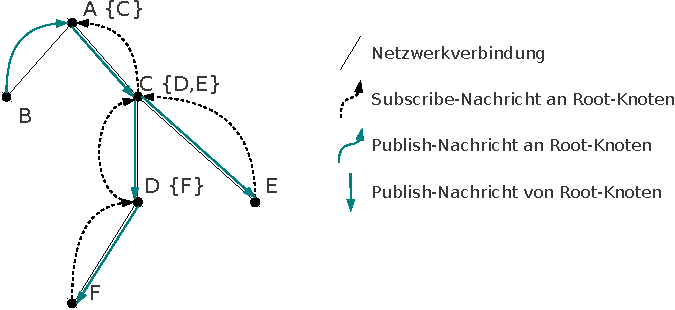
\includegraphics{grafics/multicast_tree.pdf}}
\caption{Schema eines Multicast-Trees}
\label{fig:multicast_tree}
\end{figure}

\Fref{fig:multicast_tree} zeigt ein Netzwerk mit den sechs Knoten A-F. Die Verbindungen der Knoten werden durch dünne schwarze Linien dargestellt. Beispielsweise hat Knoten C Verbindungen zu A, B, D und F.\\
Der Multicast-Tree benötigt einen Knoten, der die Wurzel (im Folgenden \emph{Root-Knoten} genannt) darstellt. Aus Hashwert des Kanalnamens wird ein Schlüssel berechnet. Derjenige Knoten, der aufgrund der Netzwerkmetrik für diesen Schlüssel zuständig ist, wird Root-Knoten des Kanals. Im abgebildeten Falle ist dies Knoten A.\\
Weiterhin hält jeder Knoten eine Liste bei ihm angemeldeter Knoten. In der Abbildung wird diese Liste durch geschweifte Klammern nach der Knotenbezeichnung dargestellt.

\paragraph{Subscribe}
Knoten F sendet eine \emph{subscribe}-Nachricht an A. Diese Nachrichten sind in der Grafik durch gebogene gestrichelte schwarze Verbindungslinien mit Pfeil dargestellt. Das Netzwerk würde diese Nachricht über Knoten D und C an A routen. Knoten D lässt die Nachricht terminieren und trägt F in die Liste der Subscriber ein. Knoten D sendet nun selbst eine subscribe-Nachricht an A. C, über den die Nachricht geroutet wird, terminiert diese, trägt D in die Liste ein und sendet selbst eine subscribe-Nachricht an A. A erhält nun diese Nachricht und trägt C in die Liste ein. Damit sind nun insgesamt drei Nachrichten verschickt worden.\\
Wenn sich Knoten E für den Kanal einschreibt, wird die subscribe-Nachricht an A über den Knoten C geleitet. Dieser terminiert die Nachricht und fügt E der Liste hinzu. Da C selbst angemeldet ist, muss keine weitere Nachricht versendet werden.

Scribe fordert periodische Anmeldungen zur Erhöhung der Fehlertoleranz. Ist ein Knoten ausgefallen, routet das Netzwerk die Nachrichten über andere Knoten. Damit kann der Multicast-Tree wieder aufgebaut werden.

\paragraph{Unsubscribe}
Der Austritt aus einem Kanal erfolgt ähnlich zur Anmeldung. Die Nachricht läuft nur bis zum nächsten Knoten und terminiert dort. Der Knoten entfernt den Sender der Nachricht aus seiner Liste und sendet selbst nur eine \emph{unsubscribe}-Nachricht, wenn die Liste leer ist und er selbst nicht angemeldet ist.

\paragraph{Publish}
In \Fref{fig:multicast_tree} möchte Knoten B eine Nachricht im Kanal publizieren. B sendet darauf eine Nachricht an den Root-Knoten A, da dieser für diesen Kanal zuständig ist (gebogene türkise Linie). Nun sendet A diese Nachricht an alle Knoten in seiner Liste (gerader türkise Linie mit Pfeil). Dies ist in der Abbildung nur Knoten C. Dieser sendet sie weiter an D und E. E gibt diese Nachricht direkt an die Applikation weiter, während D die Nachricht an F schicken muss.


Hierbei ist klar ersichtlich, dass zusätzliche Nachrichten verteilt werden müssen, wenn Knoten F eine Nachricht im Kanal publizieren möchte. Diese Nachricht muss erst von Knoten F zu Knoten A wandern, damit A diese Nachricht wieder über die anderen Knoten zurücksendet. Optimierte Versionen dieses Algorithmus können hier ansetzen und zu publizierende Nachrichten nicht mehr an den Knoten senden, der ihnen diese Nachricht geschickt hat. So würde C die Nachricht nur noch an E weiterleiten.

Bayeux \cite{Zhuang2001} ist ein ähnliches System, jedoch auf Basis des Overlay-Netzwerkes Tapestry \cite{Zhao2004Tapestry}. Tapestry entspricht auch der generischen API, somit stellt dies keinen Unterschied zu Pastry dar. Im Gegensatz zu Scribe, wird bei Bayeux der Multicast-Tree vom Root-Knoten aus aufgebaut. Aufgrund der unterliegenden Routingstruktur des genutzten Overlay-Netzwerkes können sich diese Pfade unterscheiden.


Nach diesem Einblick einer möglichen Umsetzung kanalbasiertem Publish/Subscribe, gibt der kommende Abschnitt am Beispiel von Mercury eine Vorstellung davon, wie filterbasierte Systeme\index{Publish/Subscribe!filterbasiert} in einem dezentralem Netzwerk implementiert sein können.

\subsection[Umsetzung eines filterbasierten Systemes]{Umsetzung eines filterbasierten Systemes am Beispiel von Mercury}
\label{chap:related:mercury}
Zur besseren Vorstellung einer Umsetzung für filterbasierte Publish/Subscribe-Systeme\index{Publish/Subscribe!filterbasiert} wird im folgenden Kapitel Mercury \cite{Bharambe2004Mercury} vorgestellt. Obwohl \ac{m2etis} ein kanalbasiertes Publish/Subscribe-System darstellt \cite{Fischer2010a}, ist es sinnvoll eine möglich Umsetzung eines filterbasierten Systems zu beschreiben um die grundlegenden Unterschiede der Systeme genauer auszuarbeiten. 

Im System gibt es eine Menge an Attributen, die ihrerseits einen definierten Wertebereich haben. Jedes Attribut wird durch einen eigenen Verbund aus Knoten, den sogenannten \emph{Hub}, bearbeitet. Der Wertebereich ist dabei nicht zwingend symmetrisch auf die Knoten verteilt.

\paragraph{Subscribe}
Eine Subscription $S$ ist ein Tupel aus Filterbedingungen über die Attribute (z.B. $S := (5 < x <= 20; y = 15)$) sowie Kontaktinformationen des Knotens. $S$ wird an einen beliebigen Knoten eines Hubs gesendet, der für das Attribut aus der Filterbedingung mit der größten Selektivität zuständig ist. Im Beispiel ist dies Attribut $y$. Im Hub wird $S$ nun zu dem Knoten weitergereicht, der den Wertebereich der Filterung abdeckt. Dort wird $S$ in einer Liste gespeichert.

\paragraph{Publish}
Eine Publikation $P$ ist ebenfalls ein Tupel mit bestimmten Werten der Attribute (z.B. $P := (x = 10; y = 0)$). $P$ wird an \emph{alle} Hubs gesendet und dort zum zuständigen Knoten weitergereicht. Dieser prüft nun die Liste der gespeicherten Subscriptions gegen die neue Publikation. Stimmen beide überein, so wird $P$ an den eingeschriebenen Knoten weitergeleitet.

Mirinae ist ebenfalls ein filterbasiertes Publish/Subscribe-System, stellt den Wertebereich eines Attributes jedoch als Hyperwürfel dar. Eine automatische Anpassung dieser Aufteilung ermöglicht eine schnelle Anpassung der Routingtabelle und damit einen kurzen Weg für die Nachrichten \cite{Choi2005Mirinae}.


\subsection{VON}
\label{chap:related:von}
\ac{von} ist in seinen Grundzügen stark unterschiedlich zu den bisher vorgestellen Umsetzung. \ac{von} nutzt das \ac{p2p}-Netzwerk nicht nur als Kommumnikationsmedium, sondern nutzt dessen Struktur auch als Verteilungsstruktur es Publish/Subscribe-Systems \cite{Hu2006VON}. VON zielt auf die Verteilungsoptimierung von Events zur Positonsänderun, muss allerdings über Applikationswissen verfügen: Die Position des Spielers. \ac{vast} \cite{Backhaus2007Voronoibased} greift das Konzept von \ac{von} auf und testet eine Implementierung auf OpenSIM \cite{Baumgart2007OverSim}.

\begin{figure}[htbp]
\centering
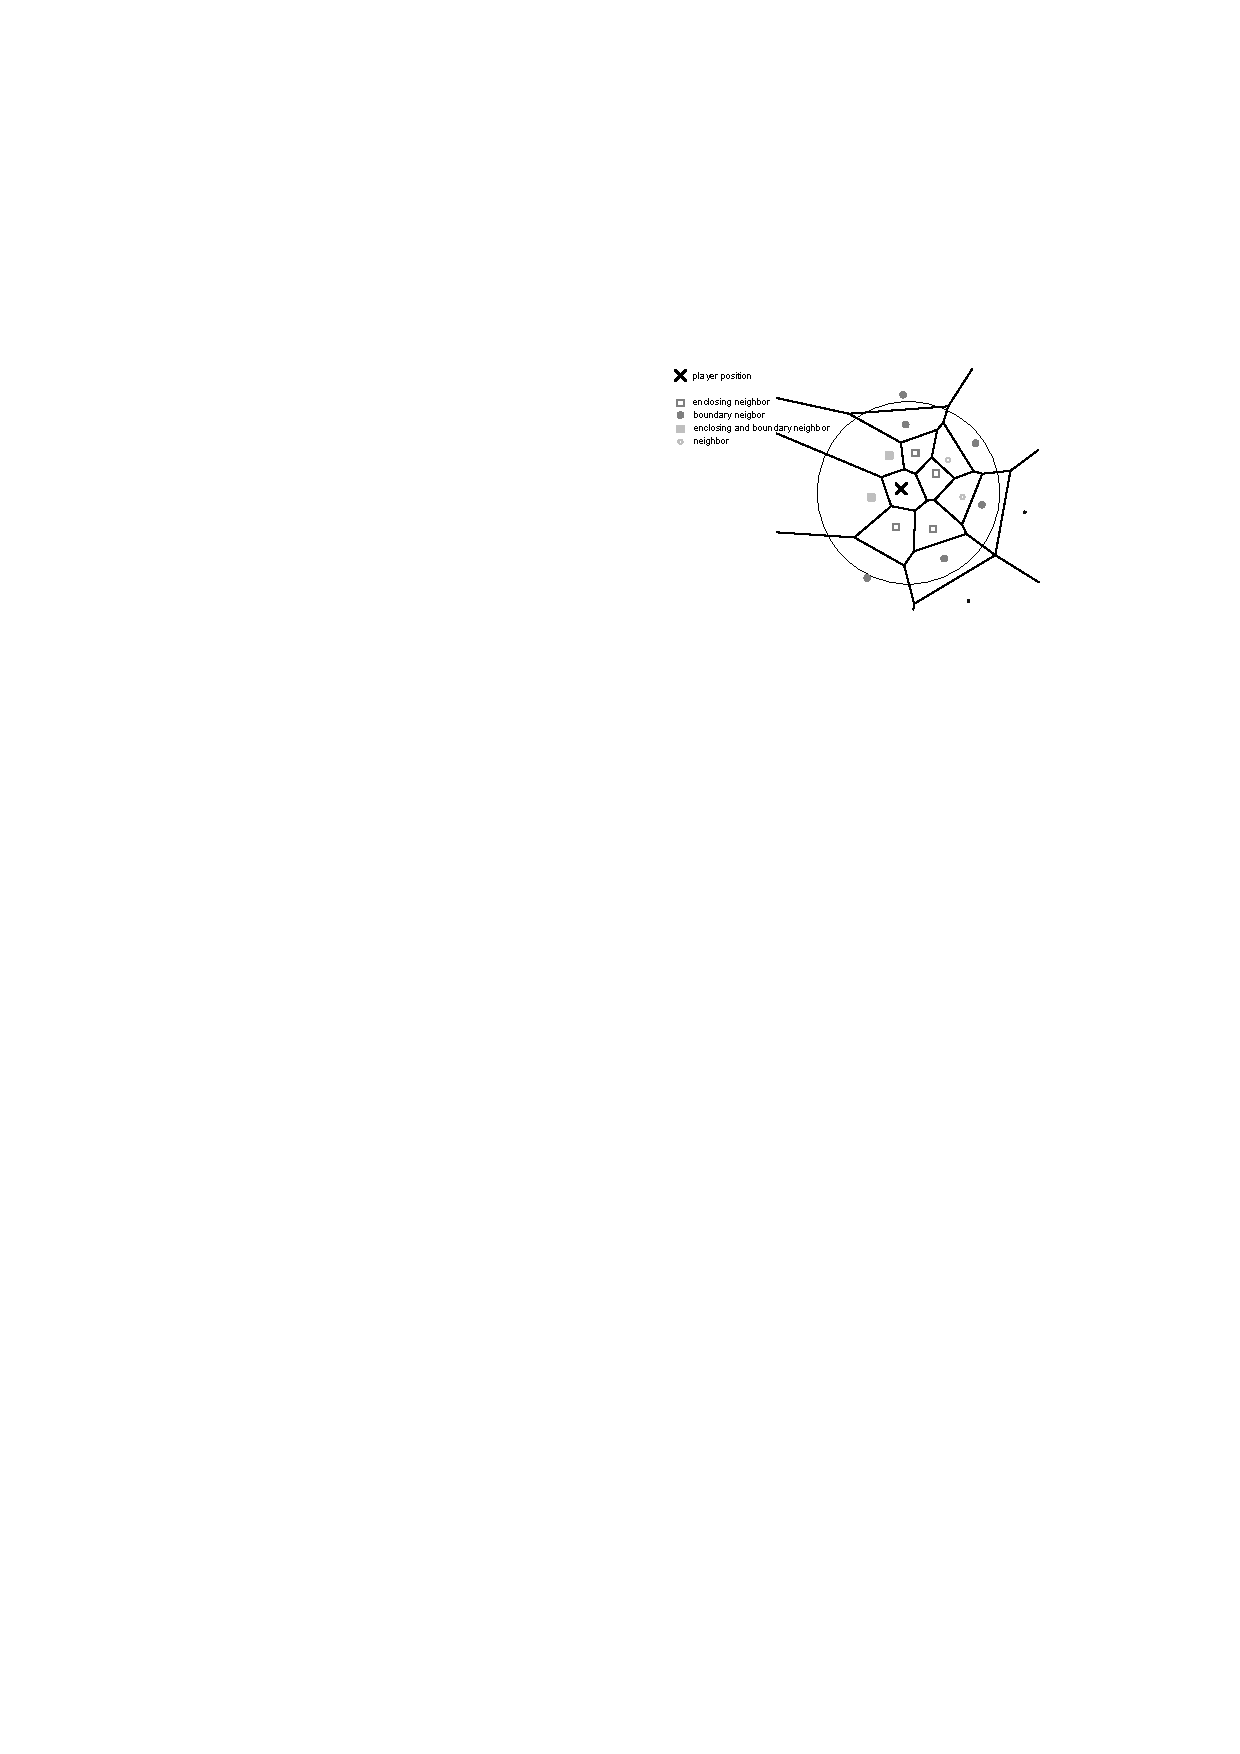
\includegraphics{grafics/voronoi_von_backhaus.pdf}
\caption{Struktur eines VON-Netzwerkes (aus \cite{Backhaus2007Voronoibased})}
\label{fig:von}
\end{figure}

\Fref{fig:von} zeigt einen Aufbau eines VON-Netzwerks. Die Spielwelt wird anhand der Position der einzelnen Knoten in Voronoi-Diagramme unterteilt. Jeder Knoten hat damit einen eigenen Bereich und hält Verbindungen zu seinen Nachbarn und kennt angrenzende Nachbarn im Bereich seiner \ac{aoi}. Anmeldungen im Publish/Subscribe-System sind implizit, denn Publikationen, also Positionsänderungen, werden von einem Knoten an alle direkt angrenzenden Nachbarn (``enclosing neighbor'' in \Fref{fig:von}) gesendet. Um das System konsistent zu halten werden dabei auch Informationen über ``boundary neighbors'' ausgetauscht.


Nach den Grundlagen von \ac{p2p}-Netzwerke, Publish/Subscribe-Systemen und Einblicke in verschiedene Umsetzungen, wird sich das nächste Kapitel mit der Evaluation dreier \ac{p2p}-Netzwerke beschäftigen und ein geeignetes System als Netzwerk für \ac{m2etis} auswählen.
